\section{Word-by-Word vs Word-by-Document Designs}
\begin{frame}{}
    \LARGE Word-by-Word vs Word-by-Document Designs
\end{frame}

\begin{frame}{Idea}
    \begin{itemize}
        \item Co-occurrence $\rightarrow$ Vector representation
        \item Relationships between words/documents
    \end{itemize}
\end{frame}

\begin{frame}{Word by Word Design}
    \begin{figure}
        \centering
        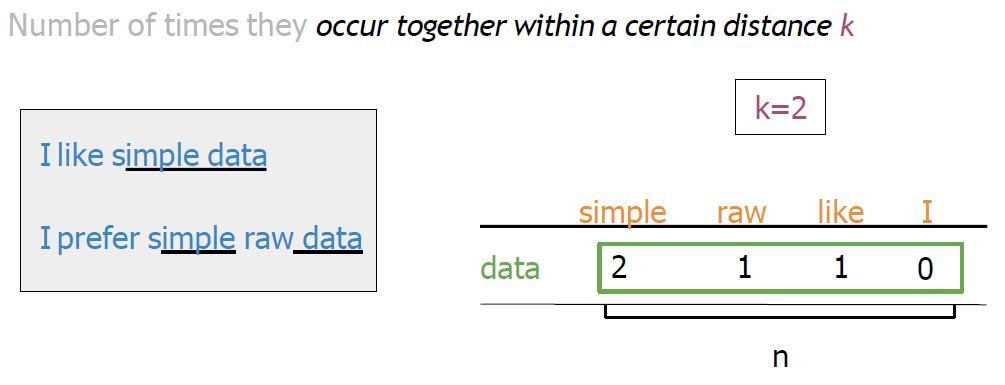
\includegraphics[width=\textwidth,height=0.8\textheight,keepaspectratio]{images/vector-space/word-by-word-design.png}
    \end{figure}
\end{frame}

\begin{frame}{Word by Document Design}
    \begin{figure}
        \centering
        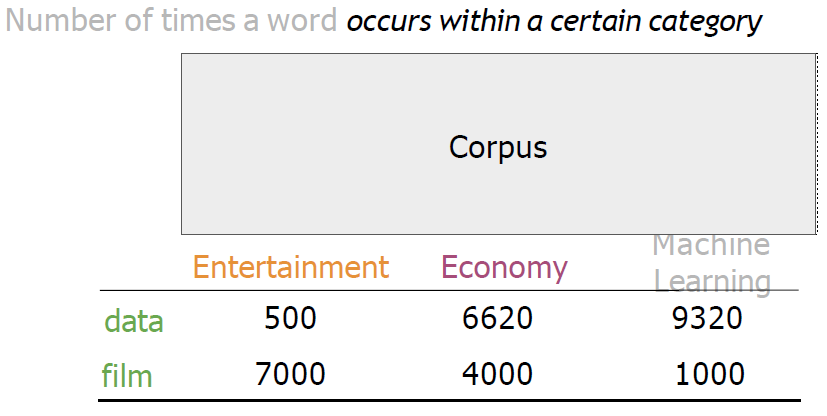
\includegraphics[width=\textwidth,height=0.8\textheight,keepaspectratio]{images/vector-space/word-by-doc-design.png}
    \end{figure}
\end{frame}

\begin{frame}{Comparison: Word-by-Word vs Word-by-Document}
    \begin{itemize}
        \item \textbf{Word-by-Word:}
        \begin{itemize}
            \item Matrix built from co-occurrence counts between words.
            \item Captures semantic similarity directly.
            \item Better for word similarity tasks.
        \end{itemize}
        \item \textbf{Word-by-Document:}
        \begin{itemize}
            \item Matrix built from word frequencies in documents.
            \item Useful for document classification and search.
            \item Better for document-level tasks.
        \end{itemize}
    \end{itemize}
    \vspace{1em}
    \textbf{Tradeoffs:} Choice depends on the task: word similarity vs. document analysis.
\end{frame}